\section{Sewer reservoir}\label{se:sewer_reservoir}
In this section the model for a reservior will be explained. 

In figure \ref{fig:tank_model} an illustration of a reservoir is shown.
\begin{figure}[H]
\centering
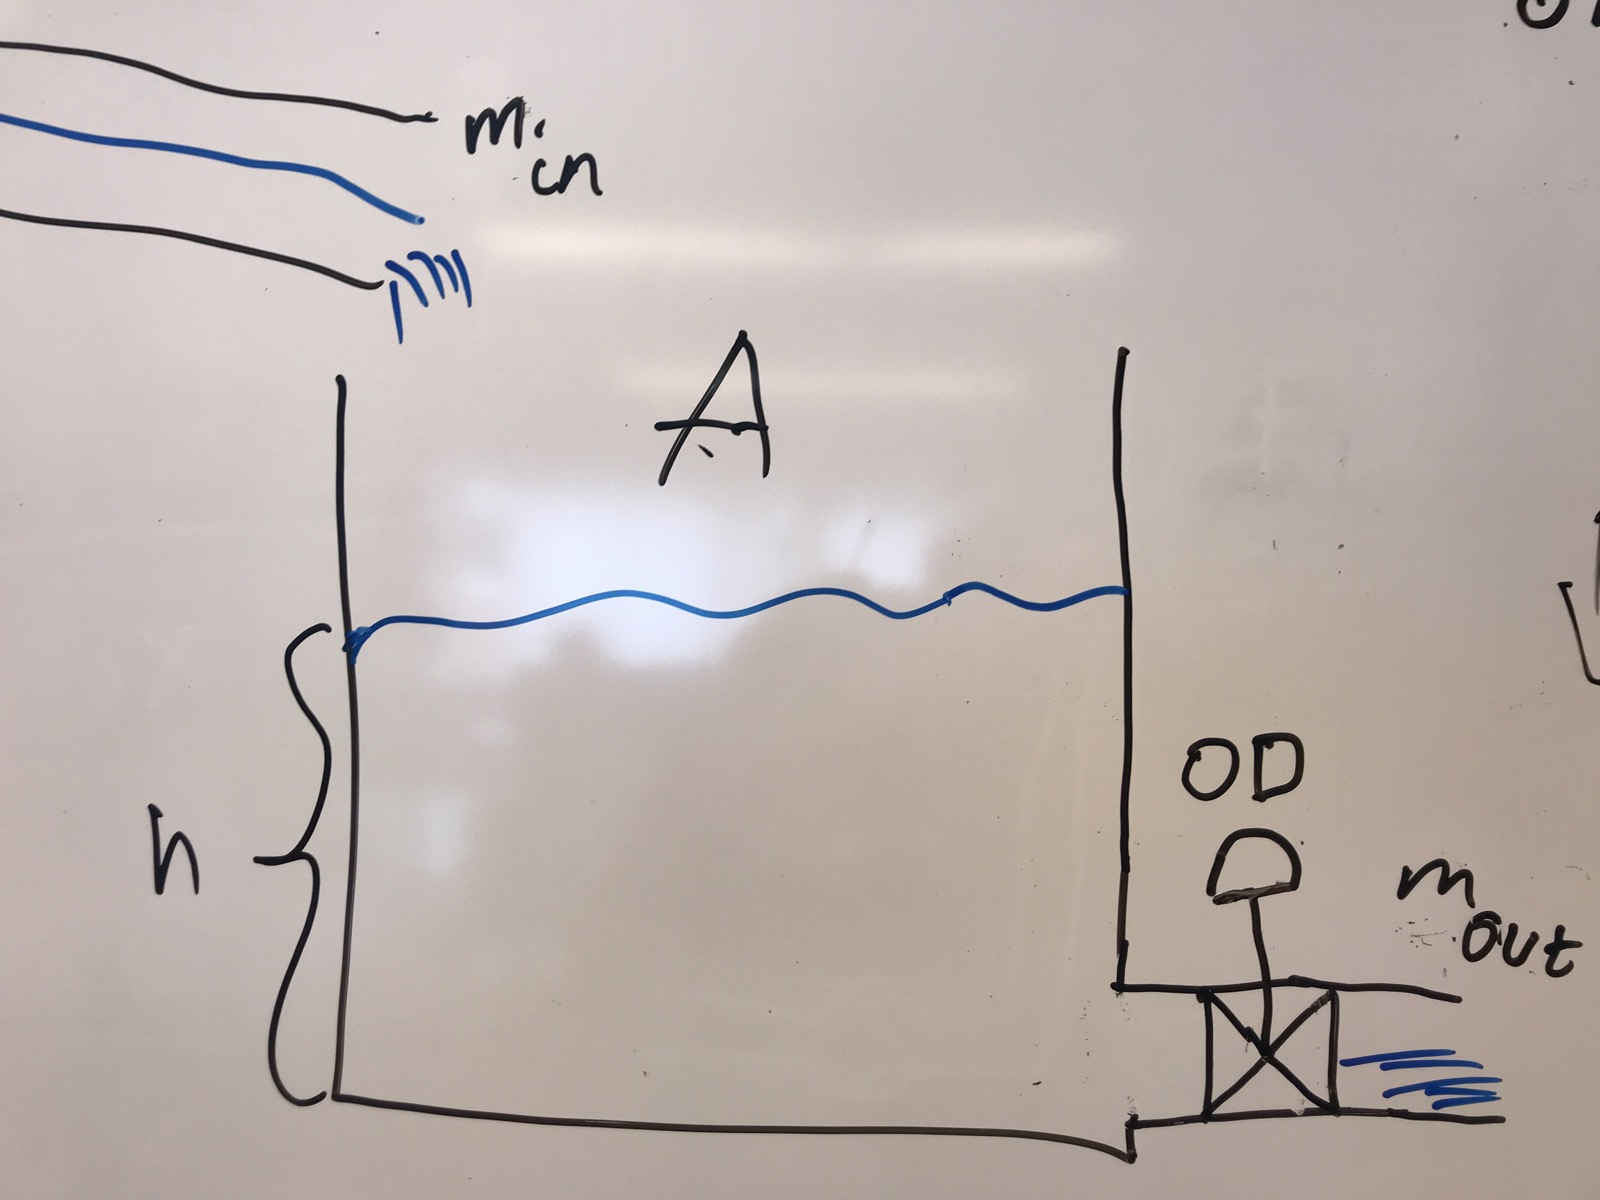
\includegraphics[width=.6\textwidth]{report/modeling/pictures/tank_model.jpg}
\caption{A illustration of a wastewater reservoir.}
\label{fig:tank_model}
\end{figure} 

This illustration will be used to derive the model for the reservior. From left we have an open channel that discharge the wastewater into the tank. The wastewater have a mass flow rate, $m_{in}$. Within the tank the wastewater has a height, h. Furhermore the reservoir has an area, A. To the bottom right the wastewater is discharged, $m_{out}$. This output mass flow is depended on the openingsdegreed (OD) of the valve. The mass balance equation is.

Assumption: incompressible flow

left side of eq: Total mass in system

\begin{equation}
	 	\frac{dM_{cv}(t)}{dt}=m_{in}(t)-m_{out}(t)
\end{equation} 

Where $M_{cv}$ is the total mass within the tank, $\left[\frac{kg}{s}\right]$, and $m_{in}$ and $m_{out}$ is the mass flow rate into the tank and away from it. Total mass balance can be written as $M_{cv} = \rho Ah$ where $\rho$ is the densisty $\left[\frac{kg}{m^3}\right]$, A is the area $\left[m^2\right]$ and h is the height [m]. The mass flow rate can be written as $m = \rho Q$, where Q is the flow $\left[\frac{m^3}{s}\right]$. Thereby the following is obtained.

\begin{equation}
		\frac{d\rho Ah(t)}{dt}=\rho Q_{in}(t)-\rho Q_{out}(t)
\end{equation}

By assuming constant densisty the following is obtained.

\begin{equation}\label{eq:balance_reservior}
	\rho A\frac{dh}{dt}=\rho \left(Q_{in}(t)-Q_{out}(t)\right)
\end{equation}
Simplifing equation \ref{eq:balance_reservior}.

\begin{equation}
	\frac{dh}{dt}=\frac{1}{A} \left(Q_{in}(t)-Q_{out}(t)\right)
\end{equation}


